\documentclass{midl}

\usepackage{booktabs}
\usepackage{multirow}
\usepackage{amsmath}
\jmlrvolume{-- Under Review}
\jmlryear{2027}
\jmlrworkshop{Full Paper -- MIDL 2027 submission}
\editors{Under Review for MIDL 2027}

\title[Directional extent supervision for lesion diameter]{Does Directional Extent Supervision Improve Lesion Diameter Agreement? A Controlled Study on Ovarian and Breast Ultrasound Masks}

\midlauthor{\Name{Nhi-Yen Nguyen-Huynh\nametag{$^{1}$}} \Email{nhinhy23411@st.uel.edu.vn}\\
\addr $^{1}$ Vietnam National University, Ho Chi Minh City -- University of Economics and Law \AND
\Name{Nguyen Quoc Khanh Le\nametag{$^{2}$}} \Email{khanhlee@tmu.edu.tw}\\
\addr $^{2}$ Taipei Medical University}

\begin{document}

\maketitle

\begin{abstract}
Segmentation models are trained and ranked by overlap, yet the lesion diameter is the quantity that is eventually read off the mask. We ask whether a measurement-preserving training term improves agreement with the maximum Feret diameter of released reference masks. The term, a \emph{directional extent loss}, projects the predicted probability mass and the reference mask onto $K$ directions, estimates differentiable upper and lower supports, and penalises normalised width differences with a robust loss. We compare it with Dice+BCE, a boundary loss and a bounding-box extent penalty, using two model families (U-Net, DeepLabV3+), three matched seeds and two public ultrasound datasets (MMOTU, ovarian; BUSI, breast), with cluster-grouped splits and a measurement protocol fixed before testing. Overlap and diameter error are only loosely coupled: Dice of 74--83\% coexists with a relative diameter error of at least 20\% in 19--29\% of test lesions. The directional loss gave \emph{no statistically supported improvement} over the strongest comparator frozen on development data (paired differences in mean relative error between $-0.008$ and $+0.006$, all 95\% group-bootstrap intervals including zero), and it inflated spurious foreground on lesion-free images. Two post-hoc revisions, one aligned with the Feret endpoint (v2) and one adding a negative-image penalty (v3), did not help either: v2 was significantly worse on MMOTU ($+0.018$ to $+0.020$), and v3 repaired the false-positive behaviour but lost the only advantage observed (fewer missed lesions) and was not better than a matched penalty-only control. We report a bounded negative result with the audit, protocol and per-case outputs needed to reproduce it. Agreement is with annotation-derived geometry, not clinical calipers.
\end{abstract}

\begin{keywords}
Ultrasound, lesion segmentation, diameter measurement, Feret diameter, differentiable geometry, negative result
\end{keywords}

\section{Introduction}

In ultrasound, a lesion is usually reported by its largest diameter rather than by its outline: ovarian lesion descriptors and breast lesion categories both rely on size \citep{timmerman2008iota,acr2013birads}. Segmentation networks, however, are trained and compared with overlap and boundary metrics \citep{ma2021loss}. Two masks with the same Dice can imply different diameters, because Dice is dominated by area while a diameter depends on the extreme points of the shape. This gap motivates training objectives that act on geometry directly, in the spirit of boundary- and distance-based losses \citep{kervadec2019boundary,karimi2020hd}, and agrees with the general argument that validation metrics must follow the target of the task \citep{maierhein2024metrics,reinke2024pitfalls}.

We ask a narrow question: \emph{does directional extent supervision reduce large errors in lesion diameter derived from released reference masks, beyond overlap, boundary and simple geometric controls, across datasets and model families?} We introduce a differentiable directional extent loss and test it in a design built so that the hypothesis can be rejected: a strong comparator set, matched tuning budgets, matched seeds, grouped evaluation, a measurement and component rule fixed before confirmation, and a decision rule stated in advance (if the loss does not help, narrow the claim).

\paragraph{Contributions.} (i) A differentiable directional extent loss with soft upper and lower supports, with numerical checks on translated shapes, elongated ellipses, distant islands, empty outputs and uniform low probabilities. (ii) A controlled comparison on MMOTU \citep{zhao2022mmotu} and BUSI \citep{aldhabyani2020busi} with two model families, a data audit and a grouped-split protocol. (iii) A bounded negative result: the loss is not distinguishable from strong baselines, has a measurable failure mode on lesion-free images, and two successive post-hoc repairs do not remove the null. (iv) Methodological findings that hold regardless of the loss: overlap does not determine measurement, small lesions drive the error tail, and the component rule changes conclusions. The study evaluates agreement with annotation-derived geometry only; clinical caliper agreement, three-dimensional size and effects on management are outside the evidence presented here.

\begin{figure}[htbp]
\floatconts
  {fig:pipeline}
  {\caption{Study pipeline (real BUSI test case, U-Net, seed 0; this case was chosen to illustrate the component rule and is not typical). \textbf{(a)} A released mask $M$ and the letterboxed image are used to train a segmenter; at test time $P$ is thresholded, the largest connected component $\mathcal{C}_{\max}$ is kept (prespecified rule; all components $\mathcal{C}_{\mathrm{all}}$ is a sensitivity analysis), and the exact maximum Feret diameter on the original grid is compared with that of $M$ (normalised absolute error, NAE). \textbf{(b)} The training-only directional extent loss compares direction-wise widths of $P$ and $M$ (hard-mask widths shown for illustration). \textbf{(c)} Frozen evaluation: paired contrasts against the comparator frozen on development data for the three variants, and the fraction of lesion-free BUSI images with any predicted foreground.}}
  {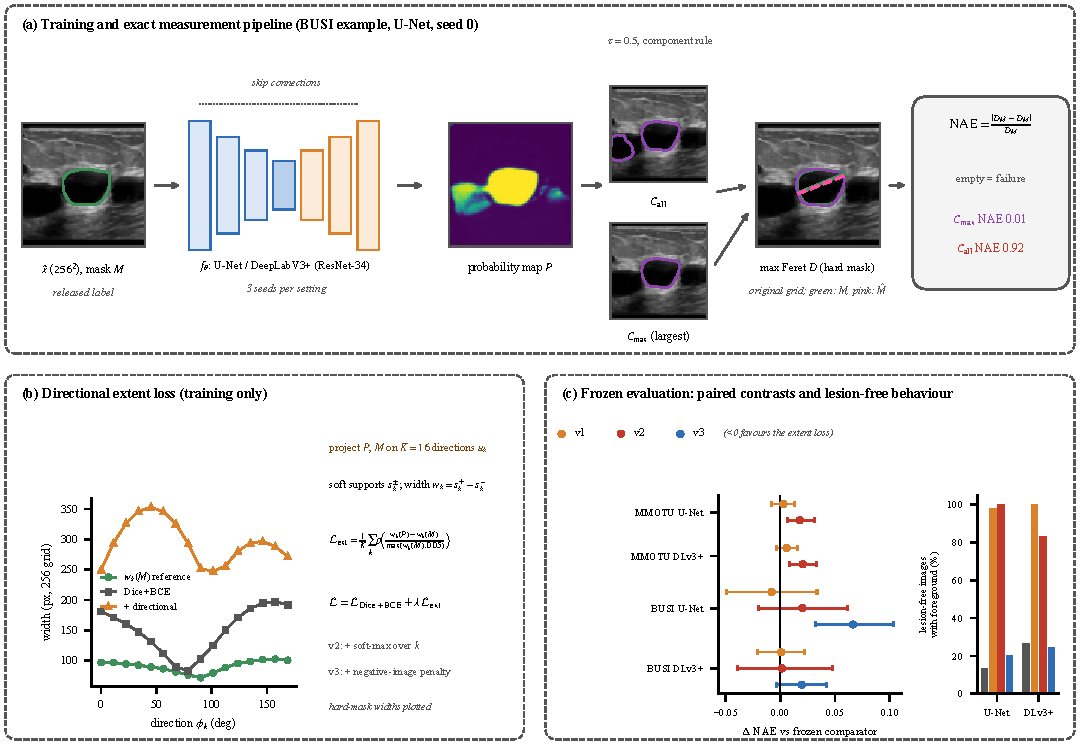
\includegraphics[width=\linewidth]{figures/pipeline.pdf}}
\end{figure}

\section{Related work}

\paragraph{Overlap and geometry-aware losses.} Dice-based and cross-entropy objectives dominate medical segmentation \citep{milletari2016vnet,isensee2021nnunet}, and large comparisons find that no single loss is uniformly best \citep{ma2021loss}. Boundary-aware terms operate on distance transforms \citep{kervadec2019boundary}, Hausdorff-distance surrogates penalise the largest boundary error \citep{karimi2020hd}, and topology-aware terms target connectivity \citep{shit2021cldice}. These act on the boundary or its topology; none targets the extent of the lesion along a measurement axis, which is what a diameter reads. Our loss belongs to this family, and our bounding-box extent penalty is its coarsest geometric control.

\paragraph{Metrics and validation.} Metric choice should follow the target of the task \citep{maierhein2024metrics,reinke2024pitfalls}, and overlap metrics are known to behave differently from distance metrics for small structures \citep{taha2015metrics}. We treat the diameter as the target and Dice only as a secondary endpoint.

\paragraph{Ultrasound lesion segmentation and measurement.} Breast ultrasound segmentation has a long literature \citep{xian2018bus}, and public sets such as BUSI \citep{aldhabyani2020busi} and the ovarian set MMOTU \citep{zhao2022mmotu} are widely used with overlap metrics. Size enters clinical rules directly \citep{timmerman2008iota,acr2013birads}, but diameter agreement derived from released masks is rarely reported alongside Dice, which is the gap studied here.

\section{Method}

\subsection{Directional extent loss}
Let $P\in[0,1]^{H\times W}$ be the predicted probability map and $M\in\{0,1\}^{H\times W}$ the reference mask. Pixel coordinates are normalised so that the longer image side spans $[-1,1]$. For each of $K$ directions $u_k=(\cos\phi_k,\sin\phi_k)$, $\phi_k=k\pi/K$, define the projection $t_k(x)=u_k^\top x$ and the soft supports
\begin{equation}\label{eq:support}
s_k^{+}(P)=\tau\log\sum_x e^{\beta(P(x)-1)}e^{t_k(x)/\tau},\qquad
s_k^{-}(P)=-\tau\log\sum_x e^{\beta(P(x)-1)}e^{-t_k(x)/\tau},
\end{equation}
with $\tau=0.02$ and $\beta=3/\tau$. The factor $e^{\beta(P-1)}$ suppresses background pixels sharply enough that a faint far-away response cannot dominate the soft maximum; a plain probability-weighted version failed our numerical checks because background mass at the image border overwhelmed the lesion. The width along $u_k$ is $w_k(P)=s_k^{+}(P)-s_k^{-}(P)$, computed identically for $M$ so that smoothing bias largely cancels. The loss is
\begin{equation}\label{eq:ext}
\mathcal{L}_{\mathrm{ext}}=\frac{1}{K}\sum_{k=1}^{K}\rho\!\left(\frac{w_k(P)-w_k(M)}{\max(w_k(M),0.05)}\right),
\end{equation}
where $\rho$ is the Huber loss \citep{huber1964robust} with $\delta=0.25$, averaged over lesion-positive images, and the total objective is $\mathcal{L}=\mathcal{L}_{\mathrm{Dice+BCE}}+\lambda\mathcal{L}_{\mathrm{ext}}$ with $K=16$. On synthetic shapes the loss is near zero for a correct or translated prediction (it constrains extent, not position), increases for a shortened ellipse (0.04) and a distant island (0.06), is large for an empty output (1.17), and has finite gradients in every case tested.

\subsection{Post-hoc variants (v2, v3)}
After the first study (v1) we examined why the loss failed. Two hypotheses followed: the mean over directions dilutes the signal from the one direction the metric measures, and training on lesion-positive images only leaves no pressure against foreground on lesion-free images.

\textbf{v2 (Feret-aligned).} A second term acts on the soft maximum over directions of the width, $\mathrm{smax}_k\,\bar w_k(P)$ with $\bar w_k=w_k/\max_j w_j(M)$ and temperature 0.05, compared with the same soft maximum applied to $M$ so that smoothing bias cancels, again with a Huber penalty; $\lambda$ multiplies the sum of both terms. In this second study, lesion-free BUSI images are included in training for \emph{all} losses and all weights are re-tuned.

\textbf{v3 (negative-aware).} The first study and v2 revealed that extent terms leave lesion-free images unconstrained. v3 adds, to the v2 objective, $\lambda_n$ times the mean of the top 1\% foreground probabilities of each lesion-free image, which pushes the maximum response to zero. To separate the effect of this penalty from that of the extent term we also train a \emph{penalty-only control}, Dice+BCE with the same penalty.

Both variants were designed after test results of the previous stage were seen; every v2 and v3 result is therefore post hoc and exploratory. Hyperparameters were chosen on development data only, and these were the only two variants tried.

\subsection{Measurement protocol}
The reference diameter is the maximum Feret diameter, the maximum distance between foreground pixel corners, computed exactly on the original image grid. Predictions are thresholded at 0.5, the largest connected component is kept (prespecified; keeping all foreground is a sensitivity analysis), and the probability map is mapped back to original geometry by removing letterbox padding and resizing before thresholding. Diameters are in pixels, so the endpoint is the \emph{relative} error $|\hat d-d|/d$, which is unit free. An empty prediction on a lesion-positive image has diameter 0 (relative error 1) and is counted as a missed lesion; failures are never excluded.

\section{Experimental design}

\subsection{Data and splits}
MMOTU \citep{zhao2022mmotu} contributes 1469 ovarian ultrasound images with released lesion masks, and BUSI \citep{aldhabyani2020busi} 780 breast images (647 with a lesion, 133 without). The official MMOTU validation list of 469 images was already used in an earlier audit of overlap versus measurement; it is therefore labelled \emph{benchmark replication}, not untouched confirmation. No patient identifiers exist in either source, so we used conservative near-duplicate clusters (difference hash, Hamming distance $\le4$) as the grouping unit; this reduces leakage risk but cannot prove patient independence. All images of a cluster stay in one split, and 19 MMOTU training images that clustered with a reserved image were dropped. BUSI was split 70/10/20 by cluster, stratified by class (Appendix~\ref{app:sup}, \tableref{tab:data}). Released labels were not edited; the audit findings (multi-component masks, merged multi-mask images, duplicates) are logged and summarised in Appendix~\ref{app:audit}.

\subsection{Models, losses and training}
We use a U-Net and a DeepLabV3+ \citep{ronneberger2015unet,chen2018deeplab} with a ResNet-34 encoder \citep{he2016resnet} initialised from ImageNet, via the segmentation\_models.pytorch library \citep{iakubovskii2019smp}. Images are letterboxed to $256\times256$ preserving aspect ratio, and models are trained for 60 epochs with AdamW \citep{loshchilov2019adamw} (learning rate $3\times10^{-4}$, one-cycle schedule, batch 16, mixed precision), flip, small affine and contrast augmentation, with final-epoch weights and no checkpoint selection. The first study trains on lesion-positive images only. The four objectives are Dice+BCE, Dice+BCE plus a boundary loss \citep{kervadec2019boundary}, plus a soft bounding-box extent penalty (the $K=2$ axis-aligned case of the same soft-support machinery), and plus the directional loss. Each added term has a three-value weight grid tuned on development data with one seed on the U-Net, so tuning budgets match; the selected weight was reused for DeepLabV3+. Final comparisons use three seeds (48 runs in the first study, 36 in v2, 12 in v3). The strongest comparator was frozen from development results before test evaluation.

\subsection{Endpoints and statistics}
The primary endpoint is the mean relative diameter error on lesion-positive test images, with seeds averaged per image. Secondary endpoints are the median, the rate of errors of at least 20\% (an operational research threshold, not a clinical one), signed bias, Dice and a boundary F1 (tolerance 2 px). We report the paired difference between the new loss and the frozen comparator with 95\% intervals from a cluster bootstrap \citep{field2007bootstrap} (5000 resamples, near-duplicate clusters resampled), per dataset and model; seed variability is reported separately. Lesion-free BUSI images are reported through the fraction with any predicted foreground and the foreground area fraction.

\section{Results}

\begin{table}[htbp]
\floatconts
  {tab:main}
  {\caption{First study: test results on lesion-positive images (mean over three seeds per image). Rel.\ err.: relative maximum-Feret error; $\ge$20: percentage of images with error $\ge0.2$; bias: signed relative error (\%); Dice and boundary F1 (\%); Missed: empty predictions per run. Bold: lowest mean error in a block. MMOTU is benchmark replication ($n=469$); BUSI $n=133$.}}
  {\scriptsize\setlength{\tabcolsep}{3pt}\begin{tabular}{llllllllll}
  \toprule
  Data & Model & Loss & Rel.\ err. & Median & $\ge$20 & Bias & Dice & BF1 & Missed\\
  \midrule
  \multirow{8}{*}{MMOTU} & \multirow{4}{*}{U-Net} & Dice+BCE & 0.162 & 0.061 & 21.5 & 3.6 & 83.1 & 24.7 & 0 \\
 &  & + Boundary & \textbf{0.157} & 0.061 & 21.0 & 2.7 & 83.0 & 24.7 & 0 \\
 &  & + BBox extent & 0.166 & 0.066 & 22.0 & 4.6 & 82.0 & 22.4 & 0 \\
 &  & + Directional (ours) & 0.160 & 0.072 & 20.6 & 2.5 & 82.5 & 24.1 & 0 \\
\midrule
 & \multirow{4}{*}{DeepLabV3+} & Dice+BCE & \textbf{0.159} & 0.067 & 20.3 & 3.8 & 82.9 & 22.4 & 0 \\
 &  & + Boundary & 0.166 & 0.067 & 21.1 & 4.5 & 82.4 & 22.1 & 0 \\
 &  & + BBox extent & 0.170 & 0.063 & 19.1 & 8.1 & 82.8 & 19.7 & 0 \\
 &  & + Directional (ours) & 0.165 & 0.066 & 19.6 & 5.9 & 82.9 & 21.8 & 0 \\
\midrule
\multirow{8}{*}{BUSI} & \multirow{4}{*}{U-Net} & Dice+BCE & 0.215 & 0.096 & 29.3 & -3.4 & 74.1 & 29.6 & 0 \\
 &  & + Boundary & 0.213 & 0.089 & 26.1 & -1.8 & 75.7 & 30.0 & 3 \\
 &  & + BBox extent & 0.214 & 0.090 & 26.1 & 3.5 & 76.6 & 25.9 & 0 \\
 &  & + Directional (ours) & \textbf{0.205} & 0.098 & 26.3 & 3.4 & 76.1 & 27.6 & 0 \\
\midrule
 & \multirow{4}{*}{DeepLabV3+} & Dice+BCE & 0.222 & 0.083 & 26.1 & 0.7 & 75.9 & 28.1 & 0 \\
 &  & + Boundary & \textbf{0.203} & 0.080 & 23.8 & 0.8 & 76.3 & 28.3 & 0 \\
 &  & + BBox extent & 0.226 & 0.097 & 28.3 & 4.5 & 75.3 & 23.0 & 0 \\
 &  & + Directional (ours) & 0.223 & 0.092 & 26.3 & 7.3 & 76.1 & 23.5 & 0 \\
  \bottomrule
  \end{tabular}}
\end{table}

\paragraph{Overlap and measurement are loosely coupled.}
\tableref{tab:main} shows Dice of 82--83\% on MMOTU and 74--77\% on BUSI, yet 19--22\% (MMOTU) and 24--29\% (BUSI) of lesions have a diameter error of at least 20\%, and the median error (6--10\%) is far below the mean (0.16--0.23): the error distribution is heavy-tailed. \figureref{fig:overlap} shows that high Dice does not exclude large diameter errors. Errors are largest for small lesions (mean 0.29--0.33 in the lowest size tertile on MMOTU against about 0.08 in the highest).

\begin{figure}[htbp]
\floatconts
  {fig:overlap}
  {\caption{Overlap versus measurement error on test lesions (U-Net, seed-averaged, error clipped at 1). The dotted line marks 20\% error.}}
  {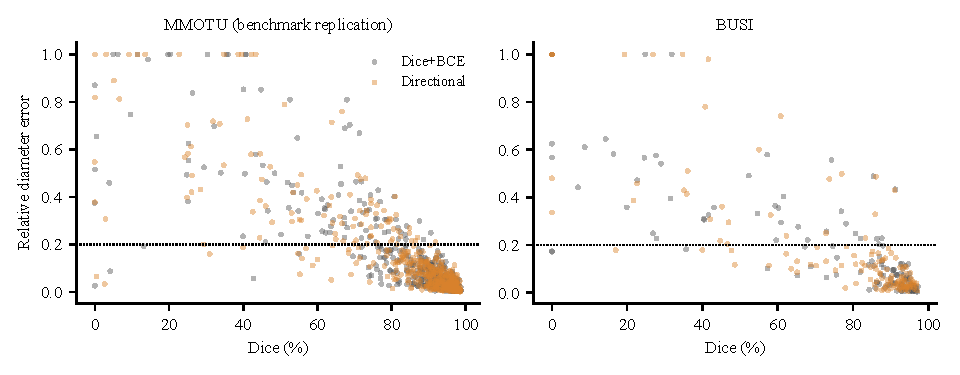
\includegraphics[width=0.78\linewidth]{figures/overlap_vs_measurement.pdf}}
\end{figure}

\paragraph{No supported benefit of the directional loss (v1).}
Against the strongest comparator frozen on development data, the paired differences in mean relative error (directional minus comparator; negative favours the directional loss) were $+0.003$ [$-0.008$, $+0.013$] (MMOTU, U-Net, boundary), $+0.006$ [$-0.004$, $+0.016$] (MMOTU, DeepLabV3+, Dice+BCE), $-0.008$ [$-0.049$, $+0.033$] (BUSI, U-Net, boundary) and $+0.001$ [$-0.021$, $+0.022$] (BUSI, DeepLabV3+, Dice+BCE). All intervals include zero, and the directional loss improved 47--51\% of individual lesions, no more than chance (Appendix~\ref{app:sup}, \tableref{tab:paired}). Dice differences were within $\pm0.6$ points with intervals spanning zero. Seed standard deviations of the mean error (0.003--0.025) are as large as most between-loss gaps, which is why a single-seed pilot on the development split (MMOTU U-Net: 0.133 for the directional loss against 0.164 for Dice+BCE) did not replicate on the test split with three seeds (0.160 against 0.162).

\paragraph{Failure modes: lesion-free images and the component rule.}
On the 30 lesion-free BUSI test images, models trained with the directional loss predicted some foreground on 100\% of images, against 76\% (U-Net) and 98\% (DeepLabV3+) for Dice+BCE, with a mean foreground area fraction of 5.6--5.8\% against 2.7--3.8\%. Since the loss is computed only on lesion-positive images and rewards extent, it pushes towards over-extension without a negative-image penalty. A related effect appears in the component sensitivity analysis: keeping all foreground instead of the largest component raised the mean BUSI error of the directional loss from 0.21 to 0.49 and of the bounding-box penalty from 0.22 to 0.59, against 0.22 to 0.31 for Dice+BCE. Extent-based terms thus benefit more from component filtering, which would make a claimed gain partly a component-rule effect. On MMOTU the rule matters little (0.16 against 0.18).

\paragraph{Post-hoc revisions (v2, v3).}
\figureref{fig:forest} and \tableref{tab:v3} summarise the second and third studies (full v2 tables in Appendix~\ref{app:v2}). On MMOTU the Feret-aligned loss was \emph{worse} than the frozen comparator: $+0.018$ [$+0.006$, $+0.031$] (U-Net) and $+0.020$ [$+0.008$, $+0.033$] (DeepLabV3+), with Dice lower by 1.7 and 1.9 points. On BUSI it was not distinguishable ($+0.020$ [$-0.020$, $+0.061$] and $+0.002$ [$-0.040$, $+0.047$]). Including lesion-free images greatly reduced spurious foreground for the baselines (13\% and 27\% of lesion-free test images with any foreground for Dice+BCE with U-Net and DeepLabV3+, against 76\% and 98\% without them), but not for the directional losses (83--100\%). The same data show the one consistent advantage we observed: Dice+BCE and the boundary loss missed 7--10 lesions per run on the BUSI test set, the directional losses 0--2, so extent terms reduce empty predictions at the price of over-extension.

The negative-aware v3 repaired the false-positive behaviour (20\% and 24\% of lesion-free images with foreground) but also lost the advantage in missed lesions (10 and 7 per run, as for the baselines). Against the frozen comparators it was $+0.066$ [$+0.032$, $+0.103$] (U-Net, bounding-box comparator) and $+0.019$ [$-0.003$, $+0.042$] (DeepLabV3+, Dice+BCE) in mean relative error, and against the penalty-only control it was not distinguishable ($-0.011$ [$-0.046$, $+0.025$] and $-0.005$ [$-0.037$, $+0.025$]); the penalty alone made Dice+BCE worse on the U-Net ($+0.078$ [$+0.034$, $+0.123$] against the bounding-box comparator). Any benefit of v3 over Dice+BCE is therefore not attributable to the extent term.

\begin{figure}[htbp]
\floatconts
  {fig:forest}
  {\caption{All paired contrasts against the comparator frozen on development data (mean relative error; negative favours the extent loss; 95\% cluster-bootstrap intervals). v1: first study; ``v1, lesion-free in training'' and v2: second study; v3: third study (BUSI only, since MMOTU has no lesion-free images). Only MMOTU v2 intervals exclude zero, in the unfavourable direction, together with BUSI U-Net v3.}}
  {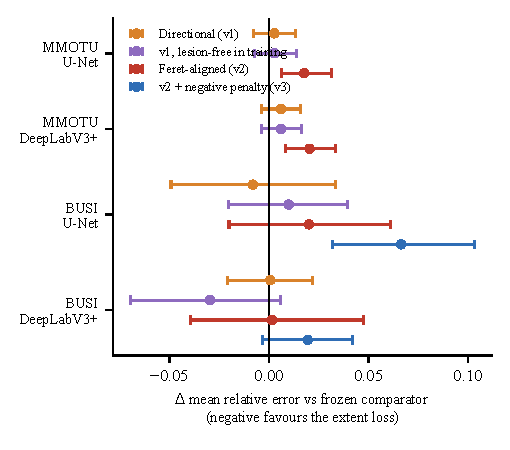
\includegraphics[width=0.78\linewidth]{figures/forest.pdf}}
\end{figure}

\begin{table}[htbp]
\floatconts
  {tab:v3}
  {\caption{Third study (post hoc), BUSI test, lesion-free images in training. Columns as in \tableref{tab:main}; FP: percentage of the 30 lesion-free test images with any predicted foreground; Area: mean foreground area fraction (\%) on those images. The penalty-only control is Dice+BCE with the same negative penalty.}}
  {\scriptsize\setlength{\tabcolsep}{3pt}\begin{tabular}{llllllllllll}
  \toprule
  Model & Loss & Rel.\ err. & Median & $\ge$20 & Bias & Dice & BF1 & Missed & FP & Area\\
  \midrule
  U-Net & Dice+BCE & 0.251 & 0.086 & 29.3 & -9.4 & 72.7 & 30.2 & 10 & 13 & 0.5 \\
U-Net & + Feret-aligned (v2) & 0.236 & 0.119 & 29.3 & 6.0 & 73.2 & 23.6 & 0 & 100 & 2.8 \\
U-Net & Dice+BCE + neg.\ penalty & 0.294 & 0.122 & 36.1 & -8.7 & 70.9 & 28.3 & 15 & 18 & 1.4 \\
U-Net & + Feret-aligned + neg.\ (v3) & 0.283 & 0.122 & 35.3 & -3.1 & 70.5 & 22.6 & 10 & 20 & 0.4 \\
\midrule
DeepLabV3+ & Dice+BCE & 0.247 & 0.082 & 28.6 & -6.3 & 74.0 & 28.2 & 8 & 27 & 0.4 \\
DeepLabV3+ & + Feret-aligned (v2) & 0.249 & 0.119 & 34.6 & 5.8 & 72.4 & 18.6 & 2 & 83 & 1.3 \\
DeepLabV3+ & Dice+BCE + neg.\ penalty & 0.272 & 0.092 & 30.8 & -5.7 & 72.0 & 25.4 & 9 & 13 & 0.5 \\
DeepLabV3+ & + Feret-aligned + neg.\ (v3) & 0.267 & 0.103 & 30.8 & -4.8 & 71.3 & 19.3 & 7 & 24 & 0.6 \\
  \bottomrule
  \end{tabular}}
\end{table}

\paragraph{Qualitative examples.}
\figureref{fig:qual} shows representative cases from the test sets. The extent losses mostly change the \emph{extent} of the predicted region rather than its location; the characteristic failure is an extended or fragmented prediction on ambiguous echogenic regions, where the largest-component rule decides the measurement.

\begin{figure}[htbp]
\floatconts
  {fig:qual}
  {\caption{Test cases (U-Net, seed 0, a re-run of the first-study configuration; green: reference mask, dashed pink: Dice+BCE, orange: directional loss, both after the component rule; text: relative diameter error). Per dataset: a typical case, the case with the largest benefit of the directional loss and the case with the largest harm. Cases were selected by their error difference, not at random.}}
  {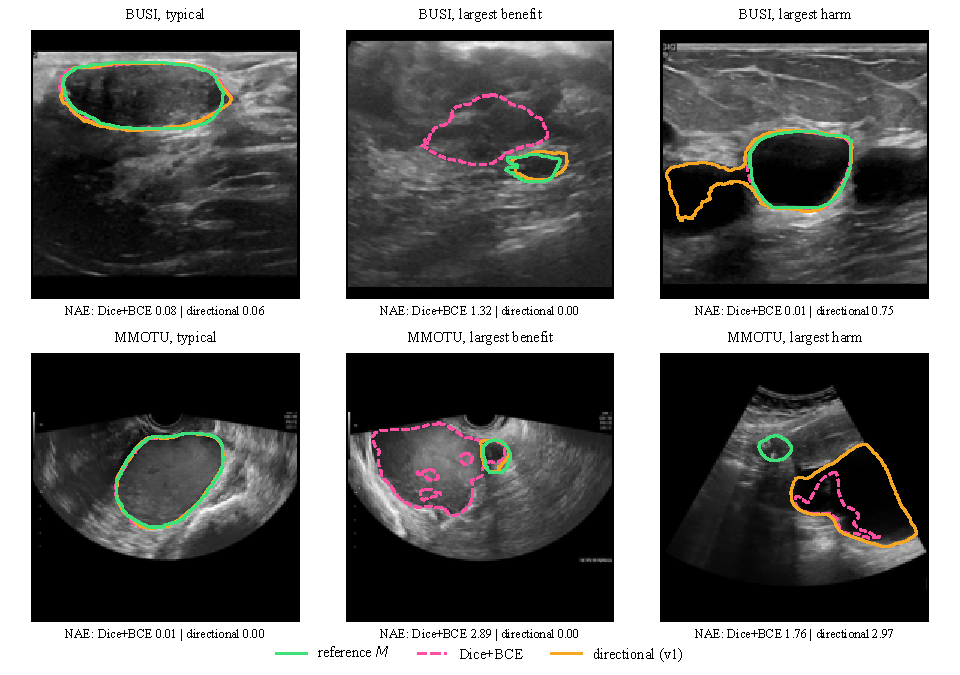
\includegraphics[width=\linewidth]{figures/qualitative.pdf}}
\end{figure}

\paragraph{Direction count.}
In a single-seed ablation, development error was lowest at $K=16$ on both datasets, consistent with the default, but test error was not monotone in $K$ (Appendix~\ref{app:K}). With one seed and differences of this size, we do not interpret the ablation as evidence for a preferred $K$.

\section{Discussion and limitations}

Under a protocol designed so that the hypothesis could fail, directional extent supervision did not improve agreement with reference-mask diameters on either dataset or model family. Following the pre-stated decision rule, this narrows the claim to a measured null result and does not support presenting the loss as a general method. Three explanations are plausible but untested: segmentation networks may already extract most of the available extent information from Dice and BCE; the remaining large errors are dominated by small and ambiguous lesions where the reference itself is uncertain; and the extent term trades missed lesions for over-extension, which a negative penalty removes together with the benefit. The post-hoc studies are informative precisely because they could have rescued the loss and did not: the same hypothesis (extent supervision helps) failed under three formulations, and v3 isolates the penalty from the extent term.

\paragraph{Limitations.} (1) Reference diameters come from released segmentation masks, not clinician calipers, so agreement says nothing about clinical measurement agreement. (2) The MMOTU test set had prior exposure and neither source has patient identifiers, so leakage control rests on near-duplicate clustering. (3) Multiple-lesion handling is limited: BUSI multi-mask images are merged by union and MMOTU instances are not separable from public metadata. (4) The tuning grid is small, and tuning used one seed and the U-Net only. (5) Results are in normalised pixel units, since pixel spacing is not available. (6) Cross-anatomy and external breast testing were not run. (7) Two model families and one encoder are a limited sample. (8) v2 and v3, the changed BUSI training set and the re-tuning were decided after test results were seen, and the MMOTU test set had prior exposure; these studies are exploratory, and although only one variant was tried at each step, a different revision could be designed with the same hindsight. (9) The qualitative figure is a re-run of one configuration, and cases are selected by error difference.

\section{Conclusion}
A differentiable directional extent loss is simple to implement and numerically stable, but in a controlled comparison on two public ultrasound datasets and two model families it did not reduce diameter error relative to strong baselines, and it increased spurious foreground on lesion-free images. A Feret-aligned revision did not help and was significantly worse on MMOTU; a negative-aware revision repaired the false positives but not the error, and was not better than a penalty-only control. The more durable results are methodological: overlap does not determine measurement, small lesions drive the tail of the error distribution, and component rules must be fixed in advance because they change conclusions. Per-case results and the measurement protocol are provided for reproduction.

\clearpage
\section*{Ethics Statement}
This study uses released research datasets and offers no clinical recommendation. No new data were collected and no patient identifiers were accessed. Images keep the licences and terms of their original sources and are not redistributed here.

\section*{Data and Code Availability}
Code, grouped split manifests, annotation issue log, frozen hyperparameters, measurement protocol and per-case results: \url{https://github.com/nhynhi23411/MIDL2027_Directional_Extent_Ultrasound}. The raw MMOTU and BUSI images are not redistributed; image identifiers and content hashes allow the splits to be rebuilt from the public releases.

\section*{Use of AI tools}
An AI assistant (Claude, Anthropic) was used to write and run analysis scripts, draft figures and edit the text under the authors' direction. The authors designed the study, checked all results and take full responsibility for the paper.

\midlacknowledgments{We thank the creators of MMOTU and BUSI for releasing their data. Funding information to be completed by the authors.}

\bibliography{refs}

\appendix
\section{Reproducibility and hyperparameters}\label{app:repro}
Code, grouped split manifests, annotation issue log, frozen hyperparameters and per-case results (one row per image, seed, model and loss) are released at the repository given in the Data and Code Availability statement. Hyperparameters selected on the development split (single seed, U-Net): weight $\lambda$ of the directional loss 1.0 (MMOTU) and 4.0 (BUSI); boundary weight 2.0 and 0.5; bounding-box weight 4.0 and 4.0. With lesion-free images in training (second study) the BUSI weights were 4.0 (directional), 4.0 (Feret-aligned), 0.5 (boundary) and 1.0 (bounding box), and 4.0 for the Feret-aligned loss on MMOTU. In the third study $\lambda=4.0$ was kept from v2 and $\lambda_n\in\{0.5,2\}$ was tuned on development data for both v3 and the penalty-only control, 0.5 being selected for both. Training took 2--7 minutes per run on a single cloud GPU (L4, T4 or A10G).

\section{Data audit}\label{app:audit}
BUSI: 780 images, of which 133 are lesion-free, 34 have multi-component masks, 22 contain tiny components, 17 have several released masks (merged by union) and 2 are exact duplicates. MMOTU: 1469 images, of which 19 have multi-component masks. All are kept and logged; none was edited.

\section{Direction-count ablation}\label{app:K}
\begin{table}[htbp]
\floatconts
  {tab:K}
  {\caption{Single-seed ablation of the number of directions $K$ for the directional loss (U-Net, mean relative error on lesion-positive images).}}
  {\small\begin{tabular}{llll}
  \toprule
  Data & $K$ & Dev & Test\\
  \midrule
  MMOTU & 4 & 0.165 & 0.167 \\
MMOTU & 8 & 0.144 & 0.160 \\
MMOTU & 16 & 0.138 & 0.154 \\
MMOTU & 32 & 0.168 & 0.159 \\
BUSI & 4 & 0.222 & 0.221 \\
BUSI & 8 & 0.207 & 0.230 \\
BUSI & 16 & 0.179 & 0.206 \\
BUSI & 32 & 0.187 & 0.245 \\
  \bottomrule
  \end{tabular}}
\end{table}

\section{Lesion-free behaviour and component sensitivity}\label{app:neg}
\begin{table}[htbp]
\floatconts
  {tab:neg}
  {\caption{BUSI test, lesion-free training (second and third studies). FP: lesion-free images with any foreground (\%); Area: mean foreground area (\%); Missed: empty predictions per run on lesion-positive images; Rel.\ err.: largest-component rule; All: keeping all foreground.}}
  {\small\begin{tabular}{lllllll}
  \toprule
  Model & Loss & FP & Area & Missed & Rel.\ err. & All\\
  \midrule
  U-Net & Dice+BCE & 13 & 0.5 & 9.7 & 0.251 & 0.298 \\
U-Net & + Boundary & 23 & 0.9 & 9.3 & 0.261 & 0.288 \\
U-Net & + BBox extent & 49 & 0.7 & 3.3 & 0.216 & 0.252 \\
U-Net & + Directional (v1) & 98 & 2.2 & 0.3 & 0.226 & 0.254 \\
U-Net & + Feret-aligned (v2) & 100 & 2.8 & 0.0 & 0.236 & 0.269 \\
U-Net & Dice+BCE + neg.\ penalty & 18 & 1.4 & 14.7 & 0.294 & 0.344 \\
U-Net & + Feret-aligned + neg.\ (v3) & 20 & 0.4 & 10.3 & 0.283 & 0.363 \\
DeepLabV3+ & Dice+BCE & 27 & 0.4 & 7.7 & 0.247 & 0.287 \\
DeepLabV3+ & + Boundary & 26 & 0.6 & 7.0 & 0.245 & 0.281 \\
DeepLabV3+ & + BBox extent & 32 & 0.7 & 7.7 & 0.248 & 0.307 \\
DeepLabV3+ & + Directional (v1) & 100 & 1.1 & 0.0 & 0.218 & 0.802 \\
DeepLabV3+ & + Feret-aligned (v2) & 83 & 1.3 & 1.7 & 0.249 & 1.922 \\
DeepLabV3+ & Dice+BCE + neg.\ penalty & 13 & 0.5 & 9.0 & 0.272 & 0.298 \\
DeepLabV3+ & + Feret-aligned + neg.\ (v3) & 24 & 0.6 & 7.3 & 0.267 & 1.274 \\
  \bottomrule
  \end{tabular}}
\end{table}

\section{Supplementary tables}\label{app:sup}
\begin{table}[htbp]
\floatconts
  {tab:data}
  {\caption{Provenance and prior exposure. Counts are lesion-positive images unless stated.}}
  {\small\begin{tabular}{lllll}
  \toprule
  Dataset & Train / dev / test & Test role & Prior exposure & Grouping\\
  \midrule
  MMOTU & 781 / 133 / 469 & benchmark replication & test set used in earlier audit & 56 multi-image clusters\\
  BUSI & 449 / 65 / 133 (+30 normal test) & held-out & none & 115 multi-image clusters\\
  \bottomrule
  \end{tabular}}
\end{table}

\begin{table}[htbp]
\floatconts
  {tab:paired}
  {\caption{First study: paired difference (directional minus frozen comparator) on test; 95\% cluster-bootstrap intervals. $\Delta$ rel.\ err.: mean relative error; \% better: lesions with lower directional error; $\Delta$ Dice in points.}}
  {\small\begin{tabular}{llllll}
  \toprule
  Data & Model & Comparator & $\Delta$ rel.\ err. [95\% CI] & \% better & $\Delta$ Dice [95\% CI]\\
  \midrule
  MMOTU & U-Net & + Boundary & +0.003 [-0.008, +0.013] & 48 & -0.5 [-1.4, +0.3] \\
MMOTU & DeepLabV3+ & Dice+BCE & +0.006 [-0.004, +0.016] & 51 & +0.0 [-0.5, +0.6] \\
BUSI & U-Net & + Boundary & -0.008 [-0.049, +0.033] & 49 & +0.4 [-1.7, +2.7] \\
BUSI & DeepLabV3+ & Dice+BCE & +0.001 [-0.021, +0.022] & 47 & +0.2 [-2.1, +2.6] \\
  \bottomrule
  \end{tabular}}
\end{table}

\section{Second-study tables}\label{app:v2}
\begin{table}[htbp]
\floatconts
  {tab:v2}
  {\caption{Second study (post hoc). Lesion-free BUSI images are included in training for all BUSI rows; the first four MMOTU losses are those of \tableref{tab:main}. Columns as in \tableref{tab:main}.}}
  {\scriptsize\setlength{\tabcolsep}{3pt}\begin{tabular}{llllllllll}
  \toprule
  Data & Model & Loss & Rel.\ err. & Median & $\ge$20 & Bias & Dice & BF1 & Missed\\
  \midrule
  \multirow{10}{*}{MMOTU} & \multirow{5}{*}{U-Net} & Dice+BCE & 0.162 & 0.061 & 21.5 & 3.6 & 83.1 & 24.7 & 0 \\
 &  & + Boundary & \textbf{0.157} & 0.061 & 21.0 & 2.7 & 83.0 & 24.7 & 0 \\
 &  & + BBox extent & 0.166 & 0.066 & 22.0 & 4.6 & 82.0 & 22.4 & 0 \\
 &  & + Directional (v1) & 0.160 & 0.072 & 20.6 & 2.5 & 82.5 & 24.1 & 1 \\
 &  & + Feret-aligned (v2) & 0.175 & 0.075 & 23.2 & 5.4 & 81.4 & 21.0 & 0 \\
\midrule
 & \multirow{5}{*}{DeepLabV3+} & Dice+BCE & \textbf{0.159} & 0.067 & 20.3 & 3.8 & 82.9 & 22.4 & 0 \\
 &  & + Boundary & 0.166 & 0.067 & 21.1 & 4.5 & 82.4 & 22.1 & 0 \\
 &  & + BBox extent & 0.170 & 0.063 & 19.1 & 8.1 & 82.8 & 19.7 & 0 \\
 &  & + Directional (v1) & 0.165 & 0.066 & 19.6 & 5.9 & 82.9 & 21.8 & 0 \\
 &  & + Feret-aligned (v2) & 0.180 & 0.077 & 21.7 & 7.1 & 81.0 & 18.1 & 0 \\
\midrule
\multirow{10}{*}{BUSI} & \multirow{5}{*}{U-Net} & Dice+BCE & 0.251 & 0.086 & 29.6 & -9.4 & 72.7 & 30.2 & 10 \\
 &  & + Boundary & 0.261 & 0.100 & 30.1 & -9.5 & 72.5 & 29.9 & 9 \\
 &  & + BBox extent & \textbf{0.216} & 0.084 & 24.8 & -4.6 & 75.1 & 29.1 & 3 \\
 &  & + Directional (v1) & 0.226 & 0.096 & 29.8 & -1.7 & 73.6 & 25.8 & 0 \\
 &  & + Feret-aligned (v2) & 0.236 & 0.119 & 30.3 & 6.0 & 73.2 & 23.6 & 0 \\
\midrule
 & \multirow{5}{*}{DeepLabV3+} & Dice+BCE & 0.247 & 0.082 & 27.6 & -6.3 & 74.0 & 28.2 & 8 \\
 &  & + Boundary & 0.245 & 0.082 & 30.1 & -8.9 & 72.7 & 27.7 & 7 \\
 &  & + BBox extent & 0.248 & 0.090 & 26.1 & -3.6 & 74.6 & 27.6 & 8 \\
 &  & + Directional (v1) & \textbf{0.218} & 0.106 & 29.3 & -1.8 & 73.1 & 22.2 & 0 \\
 &  & + Feret-aligned (v2) & 0.249 & 0.119 & 30.3 & 5.8 & 72.4 & 18.6 & 2 \\
  \bottomrule
  \end{tabular}}
\end{table}

\begin{table}[htbp]
\floatconts
  {tab:pairedv2}
  {\caption{Paired differences (new loss minus frozen comparator) in the second study; 95\% cluster-bootstrap intervals. Negative favours the new loss.}}
  {\scriptsize\begin{tabular}{lllllll}
  \toprule
  Data & Model & Loss & Comparator & $\Delta$ rel.\ err. [95\% CI] & \% better & $\Delta$ Dice [95\% CI]\\
  \midrule
  MMOTU & U-Net & + Directional (v1) & + Boundary & +0.003 [-0.007, +0.014] & 48 & -0.5 [-1.3, +0.3] \\
MMOTU & U-Net & + Feret-aligned (v2) & + Boundary & +0.018 [+0.006, +0.031] & 47 & -1.7 [-2.5, -0.8] \\
MMOTU & DeepLabV3+ & + Directional (v1) & Dice+BCE & +0.006 [-0.004, +0.016] & 51 & +0.0 [-0.5, +0.6] \\
MMOTU & DeepLabV3+ & + Feret-aligned (v2) & Dice+BCE & +0.020 [+0.008, +0.033] & 44 & -1.9 [-2.7, -1.1] \\
BUSI & U-Net & + Directional (v1) & + BBox extent & +0.010 [-0.020, +0.039] & 44 & -1.5 [-3.6, +0.4] \\
BUSI & U-Net & + Feret-aligned (v2) & + BBox extent & +0.020 [-0.020, +0.061] & 37 & -1.8 [-4.0, +0.4] \\
BUSI & DeepLabV3+ & + Directional (v1) & Dice+BCE & -0.030 [-0.070, +0.006] & 46 & -0.9 [-2.6, +0.8] \\
BUSI & DeepLabV3+ & + Feret-aligned (v2) & Dice+BCE & +0.002 [-0.040, +0.047] & 42 & -1.6 [-3.4, +0.1] \\
  \bottomrule
  \end{tabular}}
\end{table}

\begin{figure}[htbp]
\floatconts
  {fig:paired}
  {\caption{First study: per-lesion relative diameter error of the directional loss against the frozen comparator (clipped at 1). Points below the diagonal favour the directional loss; the cloud is symmetric.}}
  {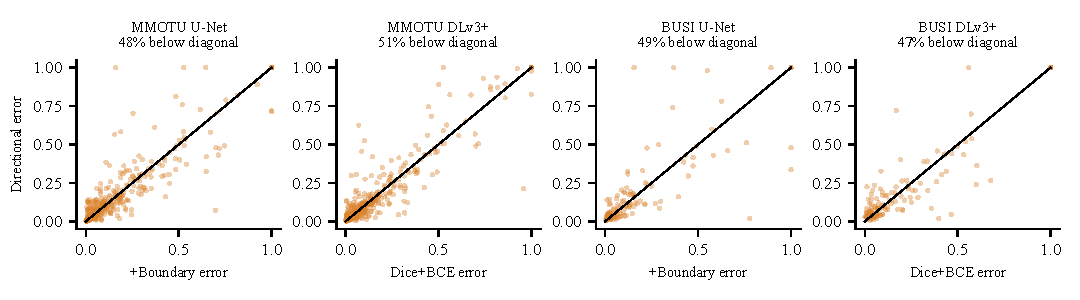
\includegraphics[width=\linewidth]{figures/paired_errors.pdf}}
\end{figure}

\section{Data use}
Both datasets are public and were used as released, under the terms set by their authors; no new data were collected and no patient identifiers were accessed.

\end{document}
